\documentclass[pdflatex,ja=standard,fleqn]{bxjsarticle}
\usepackage{ascmac,amsmath,amssymb,type1cm, tikz, graphicx}
\usetikzlibrary{intersections,calc,arrows.meta}

\title{数学IB課題1}
\author{J4-210447 川村朋広}
\begin{document}
\maketitle

\section*{1}
\begin{eqnarray*}
    \frac{d}{dx}\begin{pmatrix}
        \tilde{y_{1}} \\ \tilde{y_{2}}
    \end{pmatrix} = \begin{pmatrix}
        a \ b \\ c \ d
    \end{pmatrix}\begin{pmatrix}
        \tilde{y_{1}} \\ \tilde{y_{2}}
    \end{pmatrix}
\end{eqnarray*}
を$\tilde{y_{1}}$について変形すると、
\begin{eqnarray*}
    \tilde{y_{1}}^{\prime\prime}-(a+d)\tilde{y_{1}}^{\prime}+(ad-bc)\tilde{y_{1}} = 0
\end{eqnarray*}
となるから、固有値は$\lambda$の二次方程式、
\begin{eqnarray*}
    \lambda^{2}-(a+d)\lambda+(ad-bc)=0
\end{eqnarray*}
の2解である。2解を$\lambda_{1}$,$\lambda_{2}$とおくと、
\begin{equation}
    \left\{\,
        \begin{aligned}
            & \lambda_{1}+\lambda_{2}=a+d \\
            & \lambda_{1}\lambda_{2}=ad-bc \\
        \end{aligned}
    \right.
\end{equation}
が成り立つ。ここで、$D=(a+d)^{2}-4(ad-bc)$とおき、$D$の正負で場合分けする。\\
(a) $D>0$のとき \\
\quad$\lambda_{1}, \lambda_{2} \in \mathbb{R}$である。\\
\quad a-1) $a+d>0$かつ$ad-bc>0$のとき\\
\quad\quad$\lambda_{1}$と$\lambda_{2}$はともに正より、流れ図は総覧の(1)か(2)に対応する。\\
\quad a-2) $a+d>0$かつ$ad-bc=0$のとき\\
\quad\quad $\lambda_{1}$と$\lambda_{2}$うち、片方が$0$でもう片方が正である。したがって、流れ図は総覧の(7)に対応する。\\
\quad a-3) $a+d<=0$かつ$ad-bc>0$のとき\\
\quad\quad$\lambda_{1}$と$\lambda_{2}$はともに負より、流れ図は総覧の(3)か(4)に対応する。\\
\quad a-4) $a+d<0$かつ$ad-bc=0$のとき\\
\quad\quad$\lambda_{1}$と$\lambda_{2}$のうち、片方が$0$でもう片方は負である。したがって、流れ図は総覧の(8)に対応する。\\
\quad a-5) $ad-bc<0$のとき\\
\quad\quad$\lambda_{1}$と$\lambda_{2}$のうち片方が正でもう片方が負である。したがって、流れ図は総覧の(5)か(6)に対応する。\\\\\\\\
(b) $D=0$のとき\\
\quad$\lambda_{1}=\lambda_{2}$が成り立つ。よって、$\lambda_{1}=\lambda_{2}=\lambda_{0}$とおける。\\
\quad b-1) $a+d>0$のとき\\
\quad\quad$\lambda_{0}>0$より、流れ図は総覧の(12)に対応する。\\
\quad b-2) $a+d=0$のとき\\
\quad\quad$\lambda_{0}=0$より、$\tilde{y_{1}}=const$かつ$\tilde{y_{2}}=const$である。したがって、対応する流れ図は総覧にない。\\
\quad b-3) $a+d<0$のとき\\
\quad\quad$\lambda_{0}<0$より、流れ図は総覧の(13)に対応する\\
(c) $D<0$のとき\\
\quad$\lambda_{1}, \lambda_{2} \notin \mathbb{R}$である。$\lambda_{1}$と$\lambda_{2}$は共役より、$Re\lambda_{1}=Re\lambda_{2}=\alpha$とおける。\\
\quad c-1) $a+d>0$のとき\\
\quad\quad$\alpha>0$より、流れ図は総覧の(10)に対応する。\\
\quad c-2) $a+d=0$のとき\\
\quad\quad$\alpha=0$より、流れ図は総覧の(9)に対応する。\\
\quad c-3) $a+d<0$のとき\\
\quad\quad$\alpha<0$より、流れ図は総覧の(11)に対応する。\\
$a+d$($=X$)の値を横軸に、$ad-bc$($=Y$)の値を縦軸にとる。この平面において、領域と流れ図の対応は以下のようになる。
\begin{figure}[htbp]
    \centering
    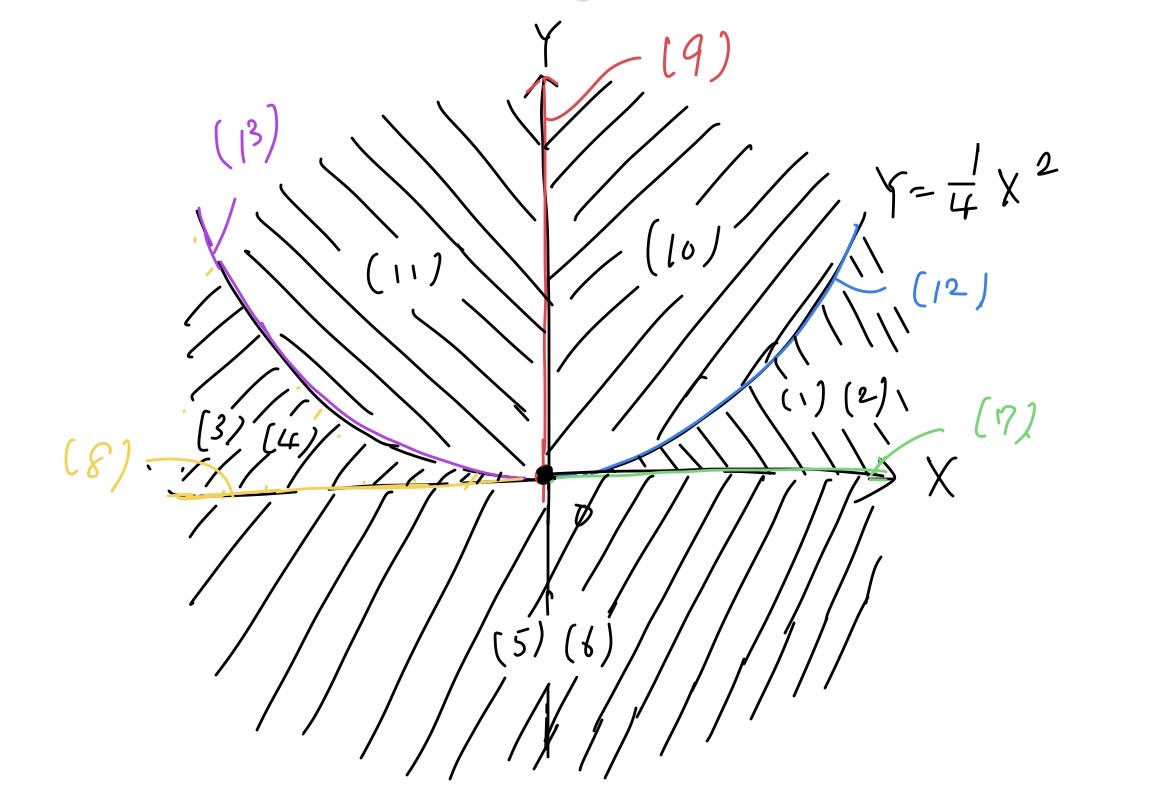
\includegraphics[width=15cm]{S__7847961.jpg}
\end{figure}
\section*{2}
(a)案出した微分方程式
\begin{eqnarray*}
    4xy^{\prime\prime}+10y^{\prime}+y=0
\end{eqnarray*}
(b)一般解の導出過程
$x=0$は確定特異点より、級数解$y$は
\begin{align*}
    & y=\sum_{k=0}^{\infty}a_{k}x^{\lambda+k}\\
    & =\sum_{k=0}^{\infty}a_{k-1}x^{\lambda+k-1}
\end{align*}
とおける。(ただし、$a_{-1}=0$)
\begin{align*}
    & y^{\prime}=\sum_{k=0}^{\infty}a_{k}(\lambda+k)x^{\lambda+k-1} \\
    & y^{\prime\prime}=\sum_{k=0}^{\infty}a_{k}(\lambda+k)(\lambda+k-1)x^{\lambda+k-2}
\end{align*}
であることより、整理すると
\begin{eqnarray*}
    \sum_{k=0}^{\infty}\left\{4a_{k}(\lambda+k)(\lambda+k+\frac{3}{2})+a_{k-1}\right\}x^{\lambda+k-1}=0
\end{eqnarray*}
となる。$k=0$とすると、$\lambda(\lambda+\frac{3}{2})=0$より、$\lambda=0, -\frac{3}{2}$である。\\
(b-1) $\lambda=0$のとき\\
$a_{k}$は漸化式
\begin{eqnarray*}
    a_{k}=-\frac{1}{2k(2k+3)}a_{k-1}
\end{eqnarray*}
をみたす。したがって、$a_{0}=a_{01}$とすると、
\begin{eqnarray*}
    a_{k} = a_{01}\prod_{l=1}^{k}\left\{-\frac{1}{2l(2l+3)}\right\}
\end{eqnarray*}
よって、基本解は
\begin{eqnarray*}
    y_{1}(x)=a_{01}\left[\sum_{k=1}^{\infty}\left\{\prod_{l=1}^{k}-\frac{1}{2l(2l+3)}\right\}x^{k}+1\right]
\end{eqnarray*}
(b-2) $\lambda=-\frac{3}{2}$のとき\\
$a_{k}$は漸化式
\begin{eqnarray*}
    a_{k}=-\frac{1}{2k(2k-3)}a_{k-1}
\end{eqnarray*}
をみたす。したがって、$a_{0}=a_{02}$とすると、
\begin{eqnarray*}
    a_{k} = a_{02}\prod_{l=1}^{k}\left\{-\frac{1}{2l(2l-3)}\right\}
\end{eqnarray*}
よって、基本解は
\begin{eqnarray*}
    y_{2}(x)=a_{02}\left[\sum_{k=1}^{\infty}\left\{\prod_{l=1}^{k}-\frac{1}{2l(2l-3)}\right\}x^{k-\frac{3}{2}}+x^{-\frac{3}{2}}\right]
\end{eqnarray*}
以上より、一般解$y$は$y_{1},y_{2}$の線形結合
\begin{eqnarray*}
    y(x)=C_{1}\left[\sum_{k=1}^{\infty}\left\{\prod_{l=1}^{k}-\frac{1}{2l(2l+3)}\right\}x^{k}+1\right]+C_{2}\left[\sum_{k=1}^{\infty}\left\{\prod_{l=1}^{k}-\frac{1}{2l(2l-3)}\right\}x^{k-\frac{3}{2}}+x^{-\frac{3}{2}}\right]
\end{eqnarray*}
と書ける。\\
(c)案出した手がかり\\
確定特異点が0より、変形した時に$y^{\prime}$と$y$の係数の分母が$x$、分子が$x=0$で定義できる関数(簡単に言うと定数)になること。また、$y^{\prime\prime}$の係数となっている関数の係数は$y^{\prime}$の係数を割り切らないこと。
\end{document}